\documentclass[aspectratio=169,10pt]{beamer}

\usetheme[progressbar=frametitle]{metropolis}
\usepackage{appendixnumberbeamer}

\usepackage{booktabs}
\usepackage[scale=2]{ccicons}

\usepackage{pgfplots}
\usepgfplotslibrary{dateplot}

\usepackage{xspace}
\newcommand{\themename}{\textbf{\textsc{metropolis}}\xspace}

\usepackage{xcolor}
\definecolor{dkgreen}{rgb}{0,0.6,0}
\definecolor{gray}{rgb}{0.5,0.5,0.5}
\definecolor{mauve}{rgb}{0.58,0,0.82}
\usepackage{listings}
\lstset{%
	numberstyle=\tiny,
	basicstyle=\fontsize{6}{8}\ttfamily,
	numbersep=15pt,tabsize=4,
	flexiblecolumns=true,
	keywordstyle=\color{blue},
	commentstyle=\color{dkgreen},
	stringstyle=\color{mauve},
	numberstyle=\tiny\color{gray},
	language=Java,
	breaklines=true,
	breakatwhitespace=true,
  showstringspaces=false,
  aboveskip=0.1em,
  belowskip=0.5em,
	morekeywords={*,num,String,var,library,get,set,StringEq,StringHashEq,bool,Top,Bot,<,String@L,String@H,int@L,int@H} ,
}


\title{DESCLASIFICACIÓN BASADA EN TIPOS EN DART}
\subtitle{IMPLEMENTACIÓN Y ELABORACIÓN DE HERRAMIENTAS DE INFERENCIA}
% \date{\today}
\date{}
\author{Matías Meneses Cortés}
%\institute{Departamento de Ciencias de la Computación}
\titlegraphic{\hfill
\includegraphics[height=2.5cm]{logo.png}}

\begin{document}

\maketitle

\begin{frame}{Contenidos}
  \setbeamertemplate{section in toc}[sections numbered]
  \tableofcontents[hideallsubsections]
\end{frame}

\section{Control de flujo de información}

\begin{frame}[fragile]{Protección de confidencialidad}
  \begin{center}
    \only<1>{
\includegraphics[width=0.8\textwidth]{images/interaccion.png}}
    \only<2>{
\includegraphics[width=0.8\textwidth]{images/interaccion2.png}}
  \end{center}
\end{frame}

\begin{frame}[fragile]{Protección de confidencialidad}
  Distintas técnicas de seguridad en distintas capas de comunicación. \pause
  \vspace{0.5cm}
  \begin{columns}[T,onlytextwidth]
    \column{0.6\textwidth}
    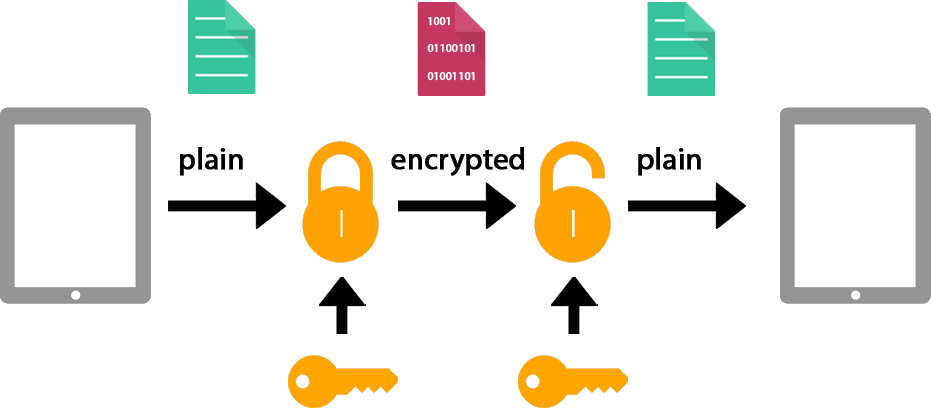
\includegraphics[width=0.8\textwidth]{images/e2e.png} \pause
    \column{0.4\textwidth}
    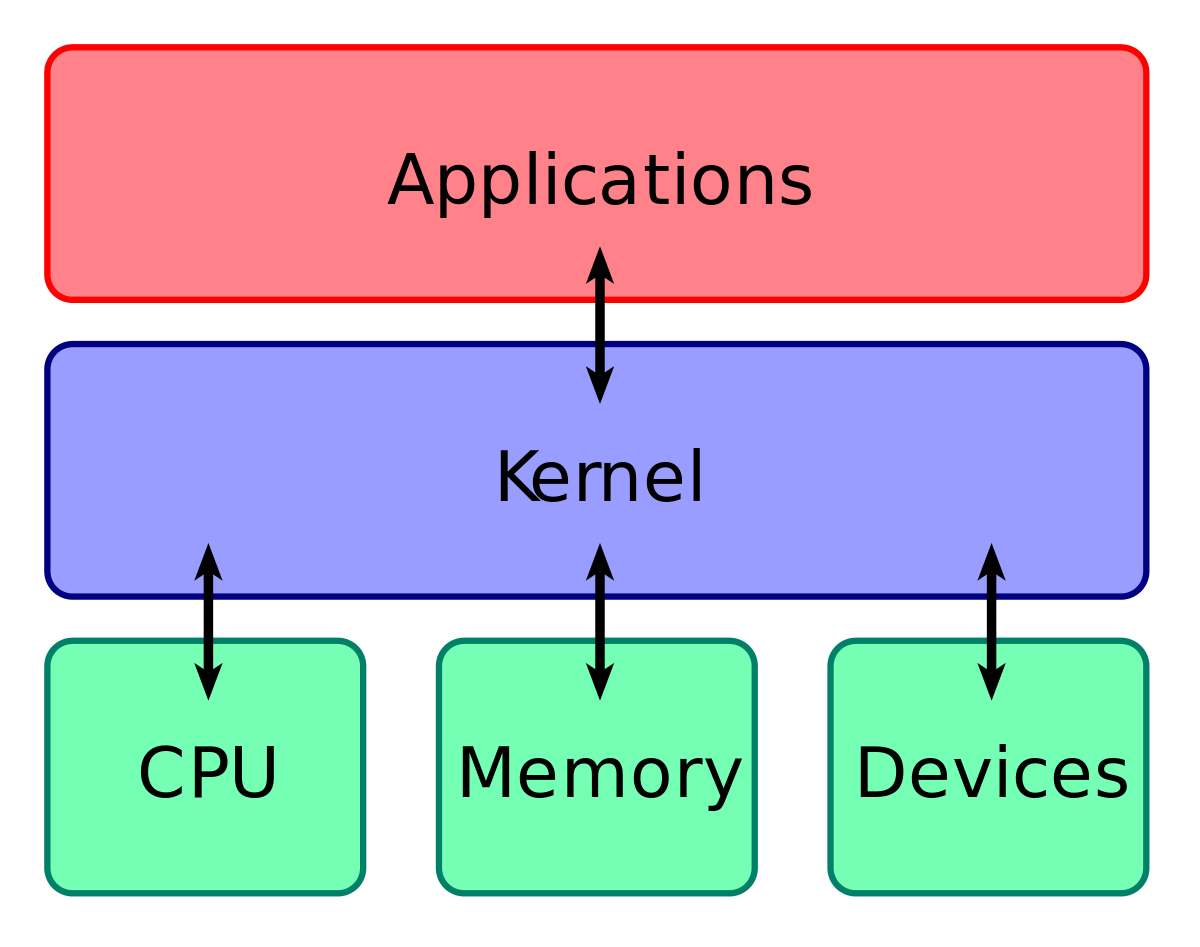
\includegraphics[width=1.0\textwidth]{images/kernel.png}
  \end{columns}
\end{frame}

\begin{frame}[fragile]{Seguridad basada en el lenguaje}
  \begin{center}
    
\includegraphics[width=0.4\textwidth]{images/lbs.png}
  \end{center}
\end{frame}

\begin{frame}[fragile]{Control de flujo de información}
  \begin{columns}[T,onlytextwidth]
    \column{0.3\textwidth}
    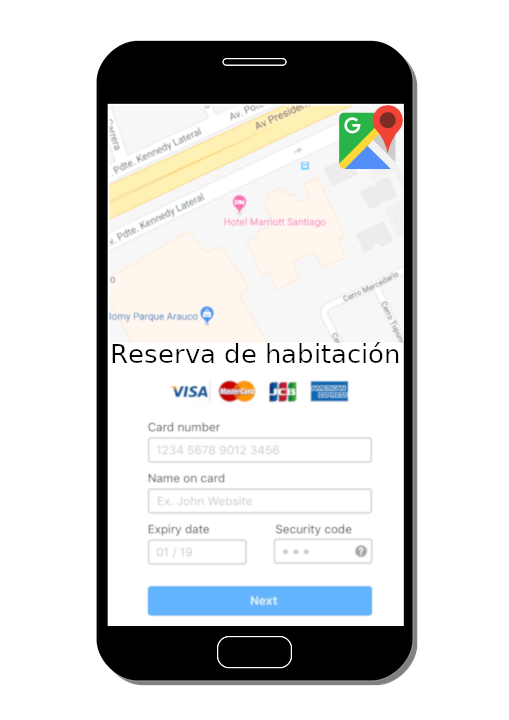
\includegraphics[width=1.0\textwidth]{images/book.png}
    \column{0.7\textwidth}
    \vspace{1cm}
    \begin{onlyenv}<1>
      \begin{lstlisting}
        String book(String username, int date, int cardNumber) {
          return sendToHotel(username, date, cardNumber);
        }

        String sendToHotel(String username, int date, int cardNumber);
        String sendToGoogle(String token, int xCoord, int yCoord);
      \end{lstlisting}
    \end{onlyenv}
    \begin{onlyenv}<2>
      \begin{lstlisting}[escapechar=?]
        String book(String username, int date, int cardNumber) {
          return ?\colorbox{yellow!50}{sendToGoogle}?(username, date, cardNumber);
        }

        String sendToHotel(String username, int date, int cardNumber);
        String sendToGoogle(String token, int xCoord, int yCoord);
      \end{lstlisting}
    \end{onlyenv}

  \end{columns}
\end{frame}

\begin{frame}[fragile]{Tipado de seguridad para el control de flujo de información}

  \begin{columns}[T,onlytextwidth]
    \column{0.3\textwidth}
    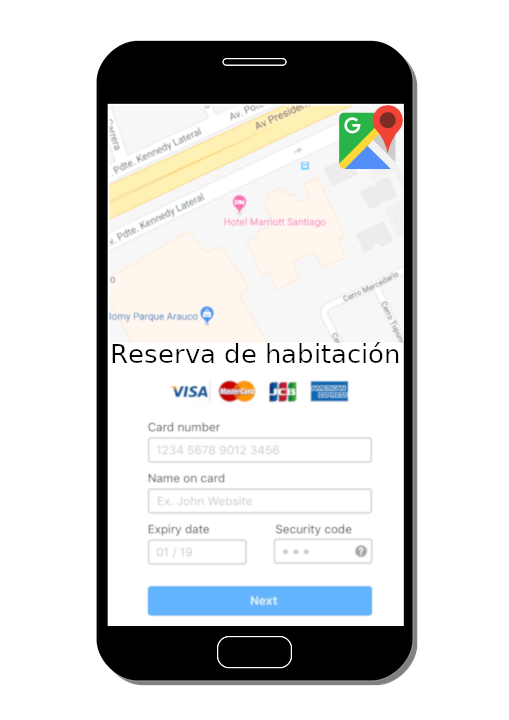
\includegraphics[width=1.0\textwidth]{images/book.png}
    \column{0.7\textwidth}
    \vspace{1cm}
    \begin{onlyenv}<1>
      \begin{lstlisting}
        String@L book(String@L username, int@L date, int@H cardNumber) {
          return sendToGoogle(username, date, cardNumber);
        }

        String@L sendToHotel(String@L username, int@L date, int@H cardNumber);
        String@L sendToGoogle(String@H token, int@L xCoord, int@L yCoord);
      \end{lstlisting}
    \end{onlyenv}
    \begin{onlyenv}<2>
      \begin{lstlisting}[escapechar=?]
        String@L book(String@L username, int@L date, int@H cardNumber) {
          ?\colorbox{red!20}{return sendToGoogle(username, date, cardNumber);}?
        }

        String@L sendToHotel(String@L username, int@L date, int@H cardNumber);
        String@L sendToGoogle(String@H token, int@L xCoord, int@L yCoord);
      \end{lstlisting}
    \end{onlyenv}
  \end{columns}

\end{frame}

\begin{frame}[fragile]{No-interferencia}
  Propiedad fundamental del control de flujo de información.
	\begin{center}
		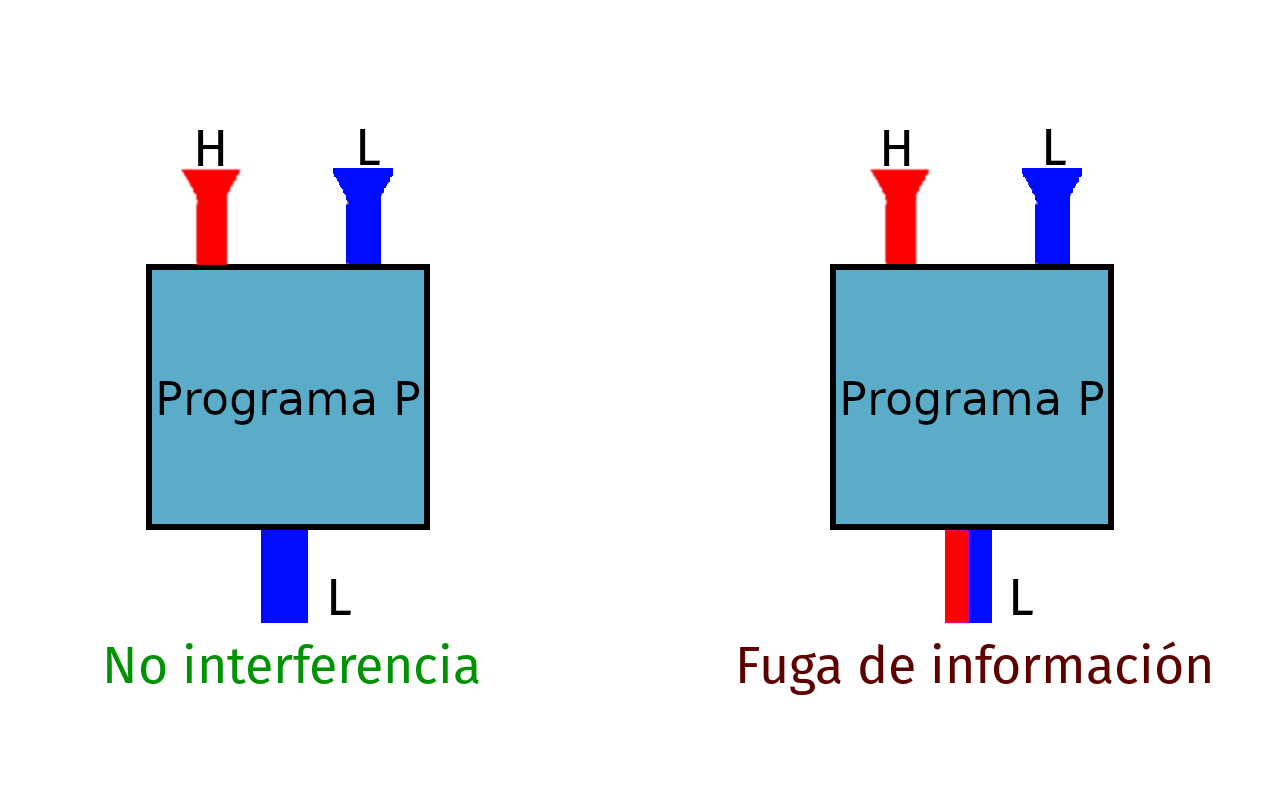
\includegraphics[width=0.8\textwidth]{images/noninterference.png}
	\end{center}

\end{frame}

\begin{frame}[fragile]{Detección de flujos explícitos inválidos}
	\begin{columns}[T,onlytextwidth]
		\column{0.33\textwidth}
		(asignación) \pause
		\column{0.33\textwidth}
		(argumento y parámetro) \pause
		\column{0.33\textwidth}
		(retorno)
	\end{columns}
\end{frame}

\begin{frame}[fragile]{Detección de flujos implícitos inválidos}
	\begin{columns}[T,onlytextwidth]
		\column{0.65\textwidth}
		\begin{onlyenv}<1>
			(codigo con if)
		\end{onlyenv}
		\begin{onlyenv}<2>
			(codigo con if y marca de pc)
		\end{onlyenv}
		\column{0.35\textwidth}

		\only<2>{Contexto de seguridad (\alert{\texttt{pc}}).}
	\end{columns}
\end{frame}

\begin{frame}[fragile]{Problema con no-interferencia}
	\begin{center}
		(Código de login) \pause \\
		\vspace{4cm}
		\alert{¡\textbf{No} cumple con no-interferencia!}
	\end{center}
\end{frame}

\begin{frame}[fragile]{Desclasificación}
	\begin{center}
		(Código de login con declassify)
	\end{center}
\end{frame}

\begin{frame}[fragile]{Problema con desclasificación}
	\begin{center}
		(Código de login con declassify(password)) \pause \\
		\vspace{4cm}
		\alert{¡Grave fuga de información!}
	\end{center}
\end{frame}

\begin{frame}[fragile]{Desclasificación basada en tipos}
	\begin{columns}[T,onlytextwidth]
		\column{0.6\textwidth}
		(código con tipos de dos facetas)
		\column{0.4\textwidth}
		\begin{itemize}
			\item \texttt{StringEq =} \\ \texttt{[eq: String -> Bool]}
			\item \texttt{String <: StringEq} \\ (Tipo bien formado)
			\item No-interferencia relajada
		\end{itemize}
	\end{columns}
\end{frame}

\begin{frame}[fragile]{Retículo de subtipos}
	\begin{center}
		(figura de reticulo)
	\end{center}
\end{frame}

\begin{frame}[fragile]{Reglas principales de la desclasificación basada en tipos}
	\begin{columns}[T,onlytextwidth]
		\column{0.5\textwidth}
		(código)
		\column{0.5\textwidth}
		\metroset{block=fill}
		\begin{block}{Métodos autorizados (TmD)}
			(regla formal)
		\end{block}
	\end{columns}
\end{frame}

\begin{frame}[fragile]{Reglas principales de la desclasificación basada en tipos}
	\begin{columns}[T,onlytextwidth]
		\column{0.5\textwidth}
		(código)
		\column{0.5\textwidth}
		\metroset{block=fill}
		\begin{block}{Métodos no autorizados (TmH)}
			(regla formal)
		\end{block}
	\end{columns}
\end{frame}

\begin{frame}[fragile]{Problemas con la desclasificación basada en tipos}
	\begin{itemize}
		\item Propuesta sin implementación práctica. \pause
		\item Anotación completa de facetas para realizar análisis. \pause
	\end{itemize}

	\begin{onlyenv}<3>
		(código con facetas públicas anotadas)
	\end{onlyenv}
	\begin{onlyenv}<4>
		(código sin facetas públicas anotadas)
	\end{onlyenv}
\end{frame}

\section{Inferencia de tipos}

\begin{frame}[fragile]{Inferencia de tipos}
	\begin{onlyenv}<1>
		(codigo con anotaciones de tipo)
	\end{onlyenv}
	\begin{onlyenv}<2>
		(codigo parcialmente anotado)
	\end{onlyenv}
\end{frame}

\begin{frame}[fragile]{Variables de tipo}
	(codigo anotado con variables de tipo)
\end{frame}

\begin{frame}[fragile]{Generación de restricciones}
	\begin{columns}[T,onlytextwidth]
		\column{0.6\textwidth}
		(codigo anotado con variables de tipo)
		\column{0.4\textwidth}
		(restricciones generadas)
	\end{columns}
\end{frame}

\begin{frame}[fragile]{Resolución de restricciones}
	(Mostrar substituciones hasta resolver)
\end{frame}

\begin{frame}[fragile]{Restricciones sobre subtipos}
	\begin{columns}[T,onlytextwidth]
		\column{0.6\textwidth}
		(codigo anotado con variables de tipo) \\
		\only<1>{(retículo de subtipos)}
		\only<2>{(retículo de subtipos mostrando meet y join)}
		\column{0.4\textwidth}
		(restricciones generadas)
	\end{columns}
\end{frame}

\begin{frame}[fragile]{Objetivo de la memoria}
	\metroset{block=fill}
	\begin{block}{Objetivo de la memoria}
		Implementar un sistema de inferencia de facetas públicas para la desclasificación basada en tipos, en conjunto con una extensión para ambientes de desarrollo.
	\end{block}
\end{frame}

\section{Inferencia de facetas públicas en Dart}

\begin{frame}[fragile]{Lenguaje Dart}
	\begin{center}
		
\includegraphics[width=0.75\textwidth]{images/dart.png}
	\end{center}
\end{frame}

\begin{frame}[fragile]{Dart Analyzer}
	\begin{center}
		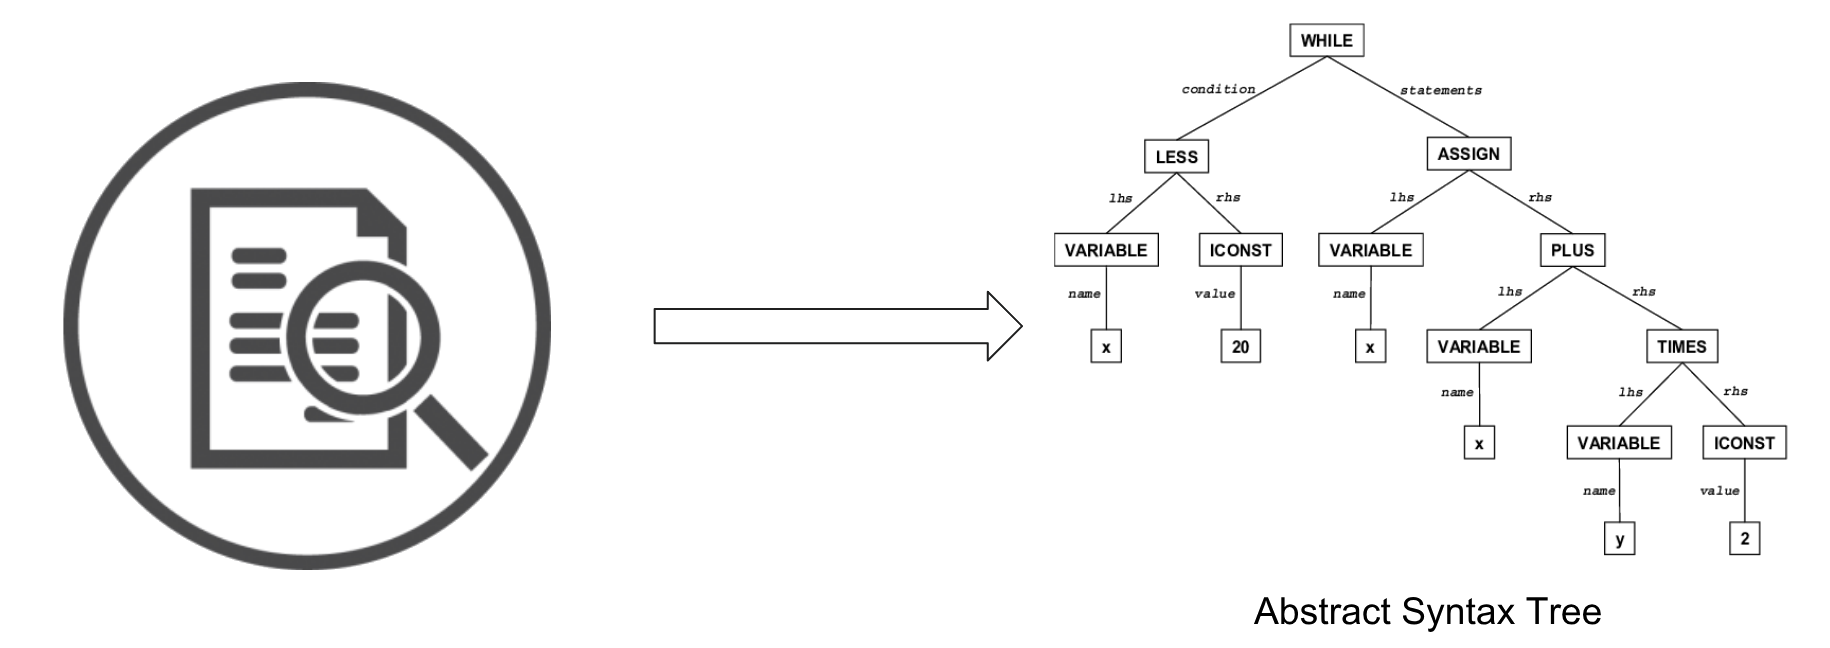
\includegraphics[width=1.0\textwidth]{images/ast.png}
	\end{center}
\end{frame}

\begin{frame}[fragile]{Analyzer Plugin}
		\begin{center}
			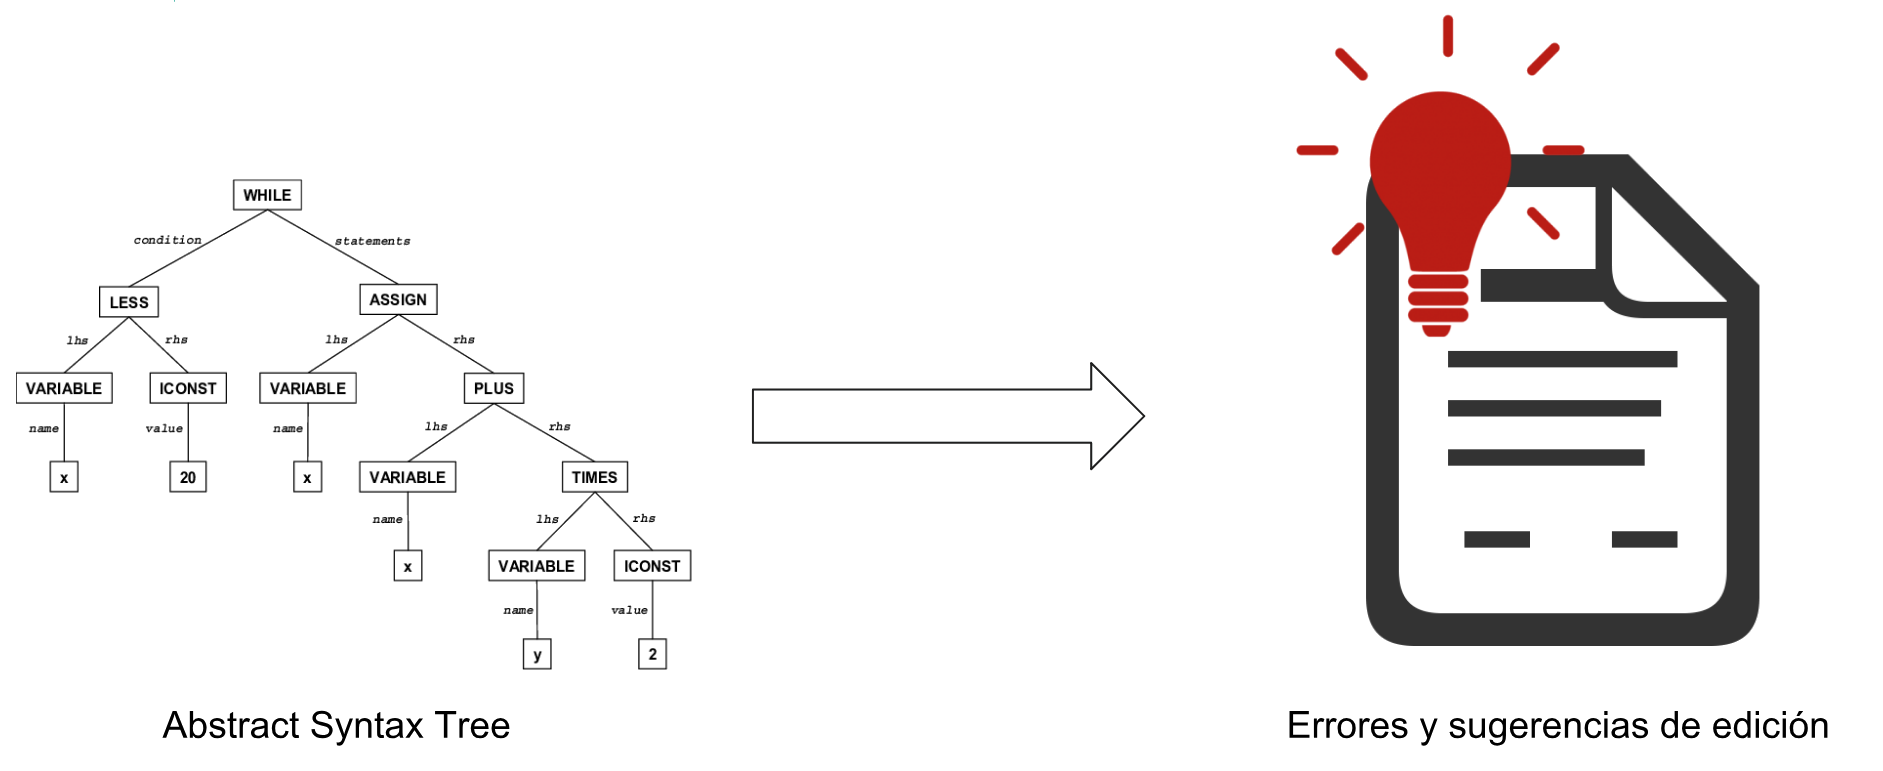
\includegraphics[width=1.0\textwidth]{images/plugin.png}
		\end{center}
\end{frame}

\begin{frame}[fragile]{Subconjunto soportado de Dart} \pause
	\begin{center}
	\begin{lstlisting}[escapechar=!,basicstyle=\fontsize{9}{11}\ttfamily]
class Foo { !\pause!
  String foo(String a, String b) { !\pause!
    String s = "foo"; !\pause!
    if (a == b)!\pause! return a.concat(b);
    return s;
  }
}
  \end{lstlisting}
	\end{center}
\end{frame}

\begin{frame}[fragile]{Problema de inferencia a resolver}
	\metroset{block=fill}
	\begin{block}{Problema de inferencia}
		Dado un programa Dart parcialmente tipado con facetas públicas, y completamente tipado con facetas privadas, encontrar la faceta pública de las expresiones no tipadas que más se ajuste al uso de las expresiones, tal que el programa sea bien tipado.
	\end{block} \pause
	\begin{onlyenv}<2>
		(código parcialmente tipado 1)
	\end{onlyenv}
	\begin{onlyenv}<3>
		(código con tipos inferidos 1)
	\end{onlyenv}
\end{frame}
\begin{frame}[fragile]{Problema de inferencia a resolver}
	\metroset{block=fill}
	\begin{block}{Problema de inferencia}
		Dado un programa Dart parcialmente tipado con facetas públicas, y completamente tipado con facetas privadas, encontrar la faceta pública de las expresiones no tipadas que más se ajuste al uso de las expresiones, tal que el programa sea bien tipado.
	\end{block}
	\begin{onlyenv}<1>
		(código parcialmente tipado 2)
	\end{onlyenv}
	\begin{onlyenv}<2>
		(código con tipos inferidos 2)
	\end{onlyenv}
\end{frame}
\begin{frame}[fragile]{Problema de inferencia a resolver}
	\metroset{block=fill}
	\begin{block}{Problema de inferencia}
		Dado un programa Dart parcialmente tipado con facetas públicas, y completamente tipado con facetas privadas, encontrar la faceta pública de las expresiones no tipadas que más se ajuste al uso de las expresiones, tal que el programa sea bien tipado.
	\end{block}
	\begin{onlyenv}<1>
		(código parcialmente tipado 3)
	\end{onlyenv}
	\begin{onlyenv}<2>
		(código con tipos inferidos 3)
	\end{onlyenv}
\end{frame}

\begin{frame}[fragile]{Declaración de facetas públicas}
	Uso de anotaciones de Dart para declarar las facetas públicas. \\ \pause

	(código con \texttt{@S("StringEq")})
\end{frame}

\begin{frame}[fragile]{Definición de facetas públicas}
	Uso de clases abstractas de Dart para declarar las facetas públicas. \\ \pause

	(código con \texttt{abstract class StringEq})
\end{frame}

\begin{frame}[fragile]{Conversión de tipos de Dart a facetas privadas}
	\begin{onlyenv}<1>
		(código donde se usan tipos definidos por el usuario y tipos de dart)
	\end{onlyenv}
	\begin{onlyenv}<2>
		(código donde se usan tipos definidos por el usuario y tipos de dart, destacando tipo definido por el usuario)
	\end{onlyenv}
	\begin{onlyenv}<3>
		(código donde se usan tipos definidos por el usuario y tipos de dart, destacando tipo estático común de dart)
	\end{onlyenv}
\end{frame}

\begin{frame}[fragile]{Conversión de tipos de Dart a facetas privadas}
	\only<1->{(Mostrar operación de convert)}\\
	\only<2>{$P_{Bi}$ (algo)}
	\only<3>{$P_{Ai}$ (algo)}

\end{frame}

\begin{frame}[fragile]{Metropolis}
  The \themename theme is a Beamer theme with minimal visual noise
  inspired by the \href{https://github.com/hsrmbeamertheme/hsrmbeamertheme}{\textsc{hsrm} Beamer
  Theme} by Benjamin Weiss.

  Enable the theme by loading

  \begin{verbatim}    \documentclass{beamer}
    \usetheme{metropolis}\end{verbatim}

  Note, that you have to have Mozilla's \emph{Fira Sans} font and XeTeX
  installed to enjoy this wonderful typography.
\end{frame}
\begin{frame}[fragile]{Sections}
  Sections group slides of the same topic

  \begin{verbatim}    \section{Elements}\end{verbatim}

  for which \themename provides a nice progress indicator \ldots
\end{frame}

\begin{frame}{Metropolis titleformats}
	\themename supports 4 different titleformats:
	\begin{itemize}
		\item Regular
		\item \textsc{Smallcaps}
		\item \textsc{allsmallcaps}
		\item ALLCAPS
	\end{itemize}
	They can either be set at once for every title type or individually.
\end{frame}

{
    \metroset{titleformat frame=smallcaps}
\begin{frame}{Small caps}
	This frame uses the \texttt{smallcaps} titleformat.

	\begin{alertblock}{Potential Problems}
		Be aware, that not every font supports small caps. If for example you typeset your presentation with pdfTeX and the Computer Modern Sans Serif font, every text in smallcaps will be typeset with the Computer Modern Serif font instead.
	\end{alertblock}
\end{frame}
}

{
\metroset{titleformat frame=allsmallcaps}
\begin{frame}{All small caps}
	This frame uses the \texttt{allsmallcaps} titleformat.

	\begin{alertblock}{Potential problems}
		As this titleformat also uses smallcaps you face the same problems as with the \texttt{smallcaps} titleformat. Additionally this format can cause some other problems. Please refer to the documentation if you consider using it.

		As a rule of thumb: Just use it for plaintext-only titles.
	\end{alertblock}
\end{frame}
}

{
\metroset{titleformat frame=allcaps}
\begin{frame}{All caps}
	This frame uses the \texttt{allcaps} titleformat.

	\begin{alertblock}{Potential Problems}
		This titleformat is not as problematic as the \texttt{allsmallcaps} format, but basically suffers from the same deficiencies. So please have a look at the documentation if you want to use it.
	\end{alertblock}
\end{frame}
}

\section{Elements}

\begin{frame}[fragile]{Typography}
      \begin{verbatim}The theme provides sensible defaults to
\emph{emphasize} text, \alert{accent} parts
or show \textbf{bold} results.\end{verbatim}

  \begin{center}becomes\end{center}

  The theme provides sensible defaults to \emph{emphasize} text,
  \alert{accent} parts or show \textbf{bold} results.
\end{frame}

\begin{frame}{Font feature test}
  \begin{itemize}
    \item Regular
    \item \textit{Italic}
    \item \textsc{SmallCaps}
    \item \textbf{Bold}
    \item \textbf{\textit{Bold Italic}}
    \item \textbf{\textsc{Bold SmallCaps}}
    \item \texttt{Monospace}
    \item \texttt{\textit{Monospace Italic}}
    \item \texttt{\textbf{Monospace Bold}}
    \item \texttt{\textbf{\textit{Monospace Bold Italic}}}
  \end{itemize}
\end{frame}

\begin{frame}{Lists}
  \begin{columns}[T,onlytextwidth]
    \column{0.33\textwidth}
      Items
      \begin{itemize}
        \item Milk \item Eggs \item Potatos
      \end{itemize}

    \column{0.33\textwidth}
      Enumerations
      \begin{enumerate}
        \item First, \item Second and \item Last.
      \end{enumerate}

    \column{0.33\textwidth}
      Descriptions
      \begin{description}
        \item[PowerPoint] Meeh. \item[Beamer] Yeeeha.
      \end{description}
  \end{columns}
\end{frame}
\begin{frame}{Animation}
  \begin{itemize}[<+- | alert@+>]
    \item \alert<4>{This is\only<4>{ really} important}
    \item Now this
    \item And now this
  \end{itemize}
\end{frame}
\begin{frame}{Figures}
  \begin{figure}
    \newcounter{density}
    \setcounter{density}{20}
    \begin{tikzpicture}
      \def\couleur{alerted text.fg}
      \path[coordinate] (0,0)  coordinate(A)
                  ++( 90:5cm) coordinate(B)
                  ++(0:5cm) coordinate(C)
                  ++(-90:5cm) coordinate(D);
      \draw[fill=\couleur!\thedensity] (A) -- (B) -- (C) --(D) -- cycle;
      \foreach \x in {1,...,40}{%
          \pgfmathsetcounter{density}{\thedensity+20}
          \setcounter{density}{\thedensity}
          \path[coordinate] coordinate(X) at (A){};
          \path[coordinate] (A) -- (B) coordinate[pos=.10](A)
                              -- (C) coordinate[pos=.10](B)
                              -- (D) coordinate[pos=.10](C)
                              -- (X) coordinate[pos=.10](D);
          \draw[fill=\couleur!\thedensity] (A)--(B)--(C)-- (D) -- cycle;
      }
    \end{tikzpicture}
    \caption{Rotated square from
    \href{http://www.texample.net/tikz/examples/rotated-polygons/}{texample.net}.}
  \end{figure}
\end{frame}
\begin{frame}{Tables}
  \begin{table}
    \caption{Largest cities in the world (source: Wikipedia)}
    \begin{tabular}{lr}
      \toprule
      City & Population\\
      \midrule
      Mexico City & 20,116,842\\
      Shanghai & 19,210,000\\
      Peking & 15,796,450\\
      Istanbul & 14,160,467\\
      \bottomrule
    \end{tabular}
  \end{table}
\end{frame}
\begin{frame}{Blocks}
  Three different block environments are pre-defined and may be styled with an
  optional background color.

  \begin{columns}[T,onlytextwidth]
    \column{0.5\textwidth}
      \begin{block}{Default}
        Block content.
      \end{block}

      \begin{alertblock}{Alert}
        Block content.
      \end{alertblock}

      \begin{exampleblock}{Example}
        Block content.
      \end{exampleblock}

    \column{0.5\textwidth}

      \metroset{block=fill}

      \begin{block}{Default}
        Block content.
      \end{block}

      \begin{alertblock}{Alert}
        Block content.
      \end{alertblock}

      \begin{exampleblock}{Example}
        Block content.
      \end{exampleblock}

  \end{columns}
\end{frame}
\begin{frame}{Math}
  \begin{equation*}
    e = \lim_{n\to \infty} \left(1 + \frac{1}{n}\right)^n
  \end{equation*}
\end{frame}
\begin{frame}{Line plots}
  \begin{figure}
    \begin{tikzpicture}
      \begin{axis}[
        mlineplot,
        width=0.9\textwidth,
        height=6cm,
      ]

        \addplot {sin(deg(x))};
        \addplot+[samples=100] {sin(deg(2*x))};

      \end{axis}
    \end{tikzpicture}
  \end{figure}
\end{frame}
\begin{frame}{Bar charts}
  \begin{figure}
    \begin{tikzpicture}
      \begin{axis}[
        mbarplot,
        xlabel={Foo},
        ylabel={Bar},
        width=0.9\textwidth,
        height=6cm,
      ]

      \addplot plot coordinates {(1, 20) (2, 25) (3, 22.4) (4, 12.4)};
      \addplot plot coordinates {(1, 18) (2, 24) (3, 23.5) (4, 13.2)};
      \addplot plot coordinates {(1, 10) (2, 19) (3, 25) (4, 15.2)};

      \legend{lorem, ipsum, dolor}

      \end{axis}
    \end{tikzpicture}
  \end{figure}
\end{frame}
\begin{frame}{Quotes}
  \begin{quote}
    Veni, Vidi, Vici
  \end{quote}
\end{frame}

{%
\setbeamertemplate{frame footer}{My custom footer}
\begin{frame}[fragile]{Frame footer}
    \themename defines a custom beamer template to add a text to the footer. It can be set via
    \begin{verbatim}\setbeamertemplate{frame footer}{My custom footer}\end{verbatim}
\end{frame}
}

\begin{frame}{References}
  Some references to showcase [allowframebreaks] \cite{knuth92,ConcreteMath,Simpson,Er01,greenwade93}
\end{frame}

\section{Conclusion}

\begin{frame}{Summary}

  Get the source of this theme and the demo presentation from

  \begin{center}\url{github.com/matze/mtheme}\end{center}

  The theme \emph{itself} is licensed under a
  \href{http://creativecommons.org/licenses/by-sa/4.0/}{Creative Commons
  Attribution-ShareAlike 4.0 International License}.

  \begin{center}\ccbysa\end{center}

\end{frame}

{\setbeamercolor{palette primary}{fg=black, bg=yellow}
\begin{frame}[standout]
  Questions?
\end{frame}
}

\appendix

\begin{frame}[fragile]{Backup slides}
  Sometimes, it is useful to add slides at the end of your presentation to
  refer to during audience questions.

  The best way to do this is to include the \verb|appendixnumberbeamer|
  package in your preamble and call \verb|\appendix| before your backup slides.

  \themename will automatically turn off slide numbering and progress bars for
  slides in the appendix.
\end{frame}

\begin{frame}[allowframebreaks]{References}

  \bibliography{defensa}
  \bibliographystyle{abbrv}

\end{frame}

\end{document}
